\tikzstyle{s} = [rectangle, rounded corners, minimum width=3cm, minimum height=1cm, text centered, draw=black, fill=white]
\tikzstyle{t} = [rectangle, rounded corners, minimum width=4cm, minimum height=1cm, text centered, draw=black, fill=gray!30]
\tikzstyle{arrow} = [thick,-,>=stealth]
\begin{center}
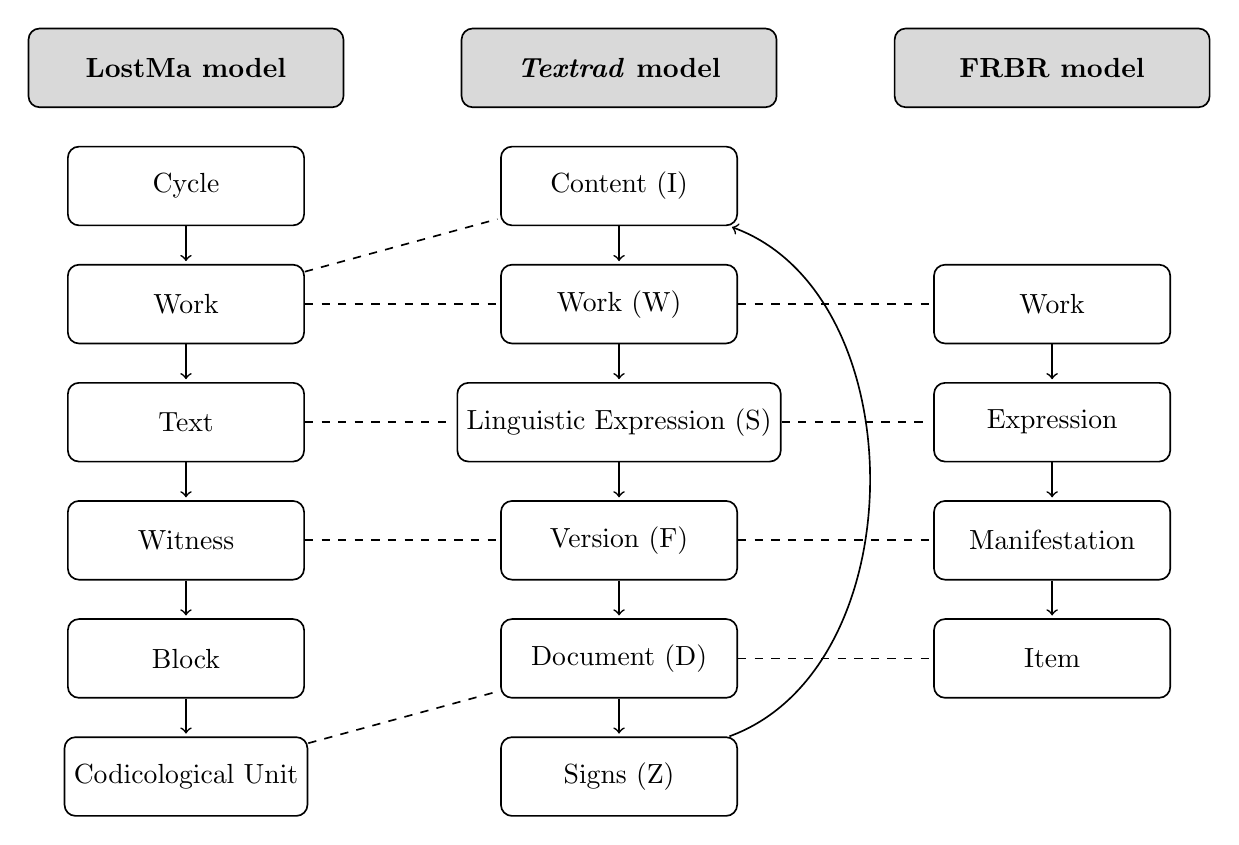
\begin{tikzpicture}[->,shorten >=1pt,auto,node distance=1.5cm,semithick]
\tikzstyle{every state}=[fill=red,draw=none,text=white]

    \node[t] (L) {\textbf{LostMa model}};
    \node[s] (LC) [below of=L]{Cycle};
    \node[s] (LWk) [below of=LC] {Work};
    \node[s] (LT) [below of=LWk] {Text};
    \node[s] (LWt) [below of=LT] {Witness};
    \node[s] (LB) [below of=LWt] {Block};
    \node[s] (LU) [below of=LB] {Codicological Unit};

    \node[t] (T) [right of=L, xshift=4cm] {\textbf{\textit{Textrad} model}};
    \node[s] (TI) [below of=T] {Content (I)};
    \node[s] (TW) [below of=TI] {Work (W)};
    \node[s] (TS) [below of=TW] {Linguistic Expression (S)};
    \node[s] (TF) [below of=TS] {Version (F)};
    \node[s] (TD) [right of=LB, xshift=4cm] {Document (D)};
    \node[s] (TZ) [below of=TD] {Signs (Z)};

    \node[t] (F) [right of=T, xshift=4cm] {\textbf{FRBR model}};
    \node[s] (FW) [right of=TW, xshift=4cm] {Work};
    \node[s] (FE) [below of=FW] {Expression};
    \node[s] (FM) [below of=FE] {Manifestation};
    \node[s] (FI) [right of=TD, xshift=4cm] {Item};

    \path[every node /.style={font=\sffamily\small}]
    (LC) edge node [right] {} (LWk)
    (LWk) edge node [right] {} (LT)
    (LT) edge node [right] {} (LWt)
    (LWt) edge node [right] {} (LB)
    (LB) edge node [right] {} (LU);

    \path[every node/.style={font=\sffamily\small}]
    (TI) edge node [right] {} (TW)
    (TW) edge node [right] {} (TS)
    (TS) edge node [right] {} (TF)
    (TF) edge node [right] {} (TD)
    (TD) edge node [right] {} (TZ)
    (TZ) edge[bend right=70] node [left] {} (TI);

    \path[every node/.style={font=\sffamily\small}]
    (FW) edge node [right] {} (FE)
    (FE) edge node [right] {} (FM)
    (FM) edge node [right] {} (FI);

    \draw[dashed, -] (LWk) -- (TW);
    \draw[dashed, -] (LWk) -- (TI);
    \draw[dashed, -] (TW) -- (FW);
    \draw[dashed, -] (LT) -- (TS);
    \draw[dashed, -] (TS) -- (FE);
    \draw[dashed, -] (LWt) -- (TF);
    % \draw[dashed, -] (LWt) -- (TS);
    \draw[dashed, -] (TF) -- (FM);
    \draw[dashed, -] (LU) -- (TD);
    \draw[dashed, -] (TD) -- (FI);

\end{tikzpicture}
\end{center}